\documentclass{beamer}
\usepackage[english, russian]{babel}
\usepackage[T2A]{fontenc}
\usepackage[utf8]{inputenc}
\usepackage{indentfirst}
\usepackage{amsmath, amsfonts, amssymb, amsthm, mathtools}
\usepackage[export]{adjustbox}
\usepackage{graphicx} 
\graphicspath{ {./images/} }

\usepackage{subcaption}
\usepackage{verbatim}

\usepackage{minted}{\setlength{\parskip}{0pt}}

\usepackage{hyperref}

\hypersetup{
    colorlinks=true,
    linkcolor=blue,
    filecolor=magenta,      
    urlcolor=black,
    pdftitle={Overleaf Example},
    pdfpagemode=FullScreen,
    }


\title{Лабораторная работа № 8. \\ Настройка SMTP-сервера}
\author{Данила Стариков \\ НПИбд-02-22}
\institute{Российский университет дружбы народов имени Патриса Лумумбы}
\date{2024}

\begin{document}

\frame{\titlepage}

\begin{frame}
\frametitle{Цель работы}
\begin{itemize}
    \item Приобретение практических навыков по установке и конфигурированию SMTP-сервера.
\end{itemize}
\end{frame}

\begin{frame}[containsverbatim]
\frametitle{Установка Postfix}
Установили необходимые для работы пакеты:
\begin{minted}{bash}
    dnf -y install postfix
    dnf -y install s-nail
\end{minted}
    \centering
    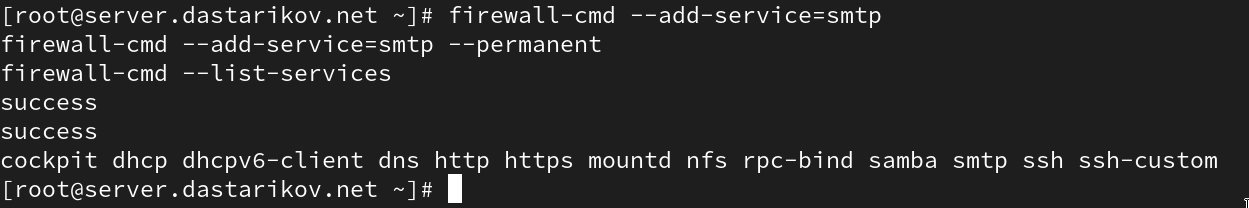
\includegraphics[width=\textwidth]{../images/image01.png}
    \captionof{figure}{Конфигурирование межсетевого экрана.}
\end{frame}
\begin{frame}
\frametitle{Установка Postfix}
    \centering
    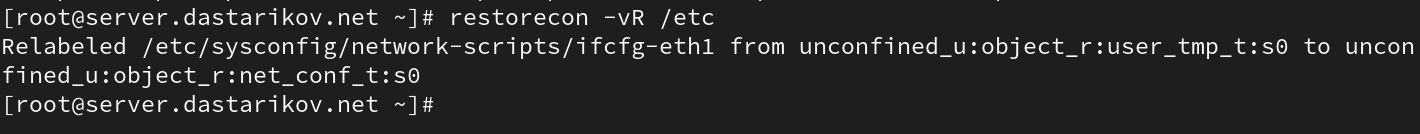
\includegraphics[width=\textwidth]{../images/image02.png}
    \captionof{figure}{Восстановление контекста безопасности SELinux.}
\end{frame}
\begin{frame}
\frametitle{Установка Postfix}
    \centering
    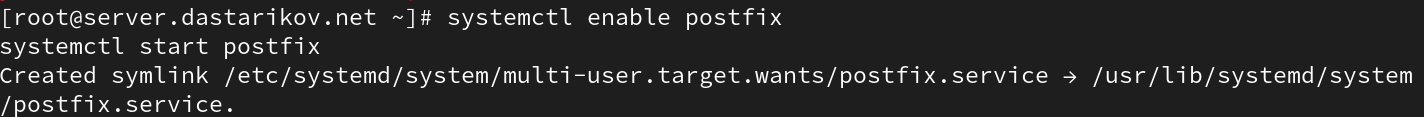
\includegraphics[width=\textwidth]{../images/image06.png}
    \captionof{figure}{Запуск службы Postfix.}
\end{frame}
\begin{frame}
\frametitle{Изменение параметров Postfix с помощью postconf}
    \centering
    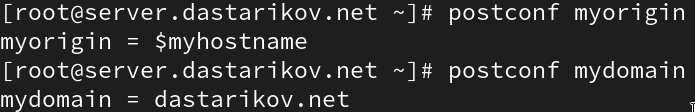
\includegraphics[width=\textwidth]{../images/image03.png}
    \captionof{figure}{Просмотр текущих настроек Postfix.}
\end{frame}
\begin{frame}
\frametitle{Изменение параметров Postfix с помощью postconf}
    \centering
    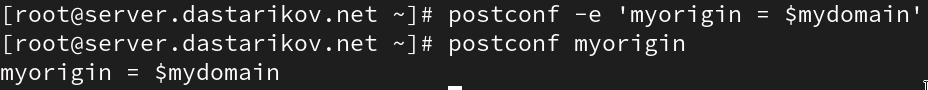
\includegraphics[width=\textwidth]{../images/image04.png}
    \captionof{figure}{Замена значений параметров Postfix.}
\end{frame}
\begin{frame}
\frametitle{Изменение параметров Postfix с помощью postconf}
    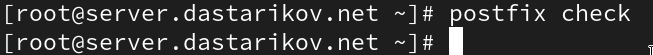
\includegraphics[width=\textwidth]{../images/image05.png}
    \captionof{figure}{Проверка корректности содержания конфигурационного файла \texttt{main.cf}.}
\end{frame}
\begin{frame}
\frametitle{Изменение параметров Postfix с помощью postconf}
    \centering
    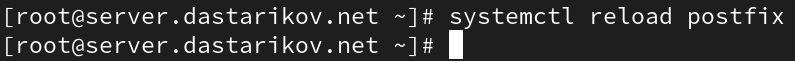
\includegraphics[width=\textwidth]{../images/image07.png}
    \captionof{figure}{Перезагрузка службы Postfix.}
\end{frame}
\begin{frame}
\frametitle{Изменение параметров Postfix с помощью postconf}
    \centering
    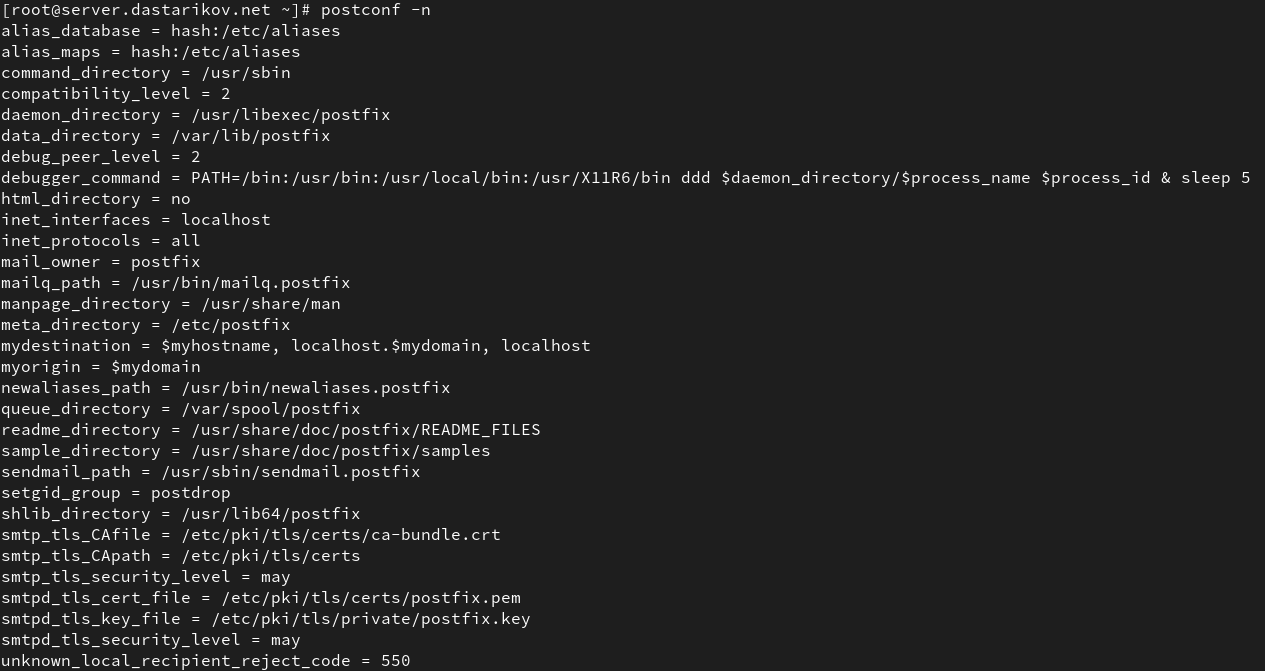
\includegraphics[width=\textwidth]{../images/image08.png}
    \captionof{figure}{Просмотр всех параметров Postfix с отличиями от начальных.}
\end{frame}
\begin{frame}
\frametitle{Изменение параметров Postfix с помощью postconf}
    \centering
    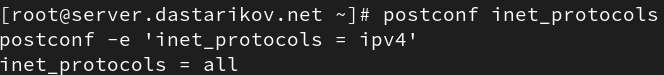
\includegraphics[width=\textwidth]{../images/image09.png}
    \captionof{figure}{Настройка Postfix на работу только с протоколом IPv4.}
\end{frame}
\begin{frame}
\frametitle{Изменение параметров Postfix с помощью postconf}
    \centering
    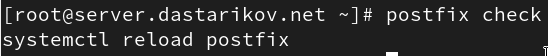
\includegraphics[width=\textwidth]{../images/image10.png}
    \captionof{figure}{Перезагрузка службы Postfix.}
\end{frame}
\begin{frame}[containsverbatim]
\frametitle{Проверка работы Postfix}
  \begin{minted}{bash}
    echo .| mail -s test1 dastarikov@server.dastarikov.net
  \end{minted}
    \centering
    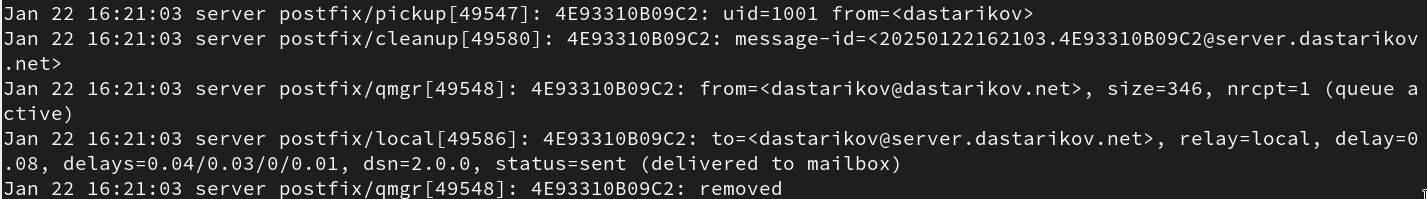
\includegraphics[width=\textwidth]{../images/image11.png}
    \captionof{figure}{Просмотр логов почтовой службы при отправке сообщения.}
\end{frame}
\begin{frame}
\frametitle{Проверка работы Postfix}
    \centering
    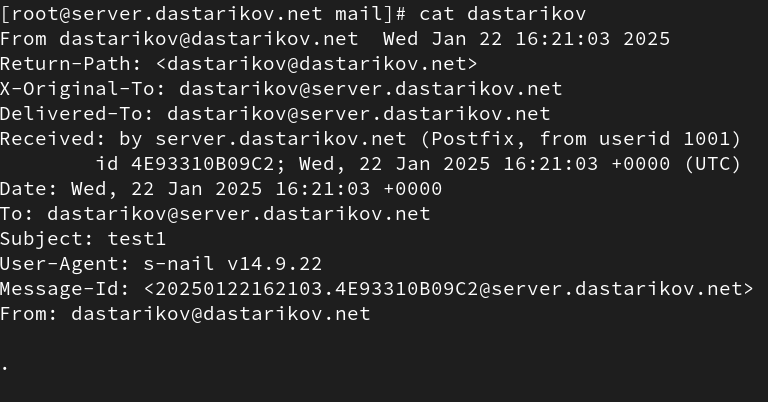
\includegraphics[width=\textwidth]{../images/image12.png}
    \captionof{figure}{Содержимое отправленного сообщения.}
\end{frame}
\begin{frame}[containsverbatim]
\frametitle{Проверка работы Postfix}
Установили необходимые для работы пакеты:
  \begin{minted}{bash}
    dnf -y install postfix
    dnf -y install s-nail
  \end{minted}
    \centering
    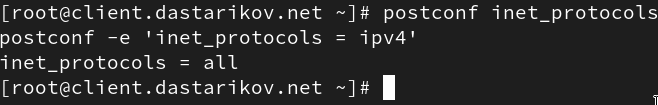
\includegraphics[width=\textwidth]{../images/image13.png}
    \captionof{figure}{Настройка Postfix на работу только с протоколом IPv4 на клиенте.}
\end{frame}
\begin{frame}
\frametitle{Проверка работы Postfix}
    \centering
    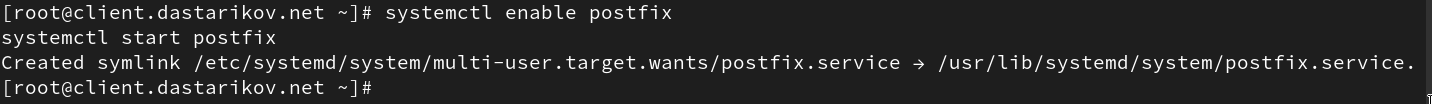
\includegraphics[width=\textwidth]{../images/image14.png}
    \captionof{figure}{Перезапуск службы Postfix.}
\end{frame}
\begin{frame}
\frametitle{Проверка работы Postfix}
    \centering
    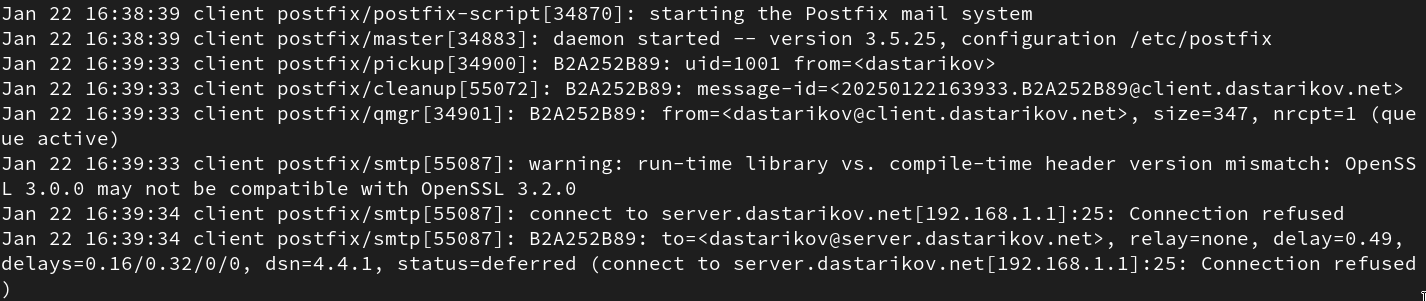
\includegraphics[width=\textwidth]{../images/image15.png}
    \captionof{figure}{Логи при попытке отправить сообщение с клиента.}
\end{frame}
\begin{frame}
\frametitle{Проверка работы Postfix}
    \centering
    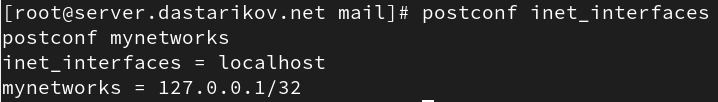
\includegraphics[width=\textwidth]{../images/image16.png}
    \captionof{figure}{Просмотр значений параметров сетевых интерфейсов.}
\end{frame}
\begin{frame}
\frametitle{Проверка работы Postfix}
    \centering
    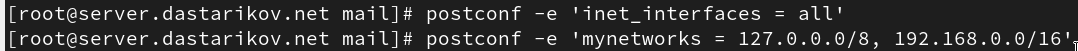
\includegraphics[width=\textwidth]{../images/image17.png}
    \captionof{figure}{Добавление адреса внутренней сети для разрешения пересылки сообщений между узлами сети.}
\end{frame}
\begin{frame}
\frametitle{Проверка работы Postfix}
    \centering
    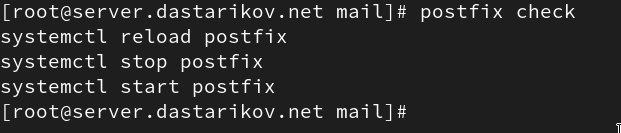
\includegraphics[width=\textwidth]{../images/image18.png}
    \captionof{figure}{Перезагрузка службы Postfix.}
\end{frame}
\begin{frame}
\frametitle{Проверка работы Postfix}
    \centering
    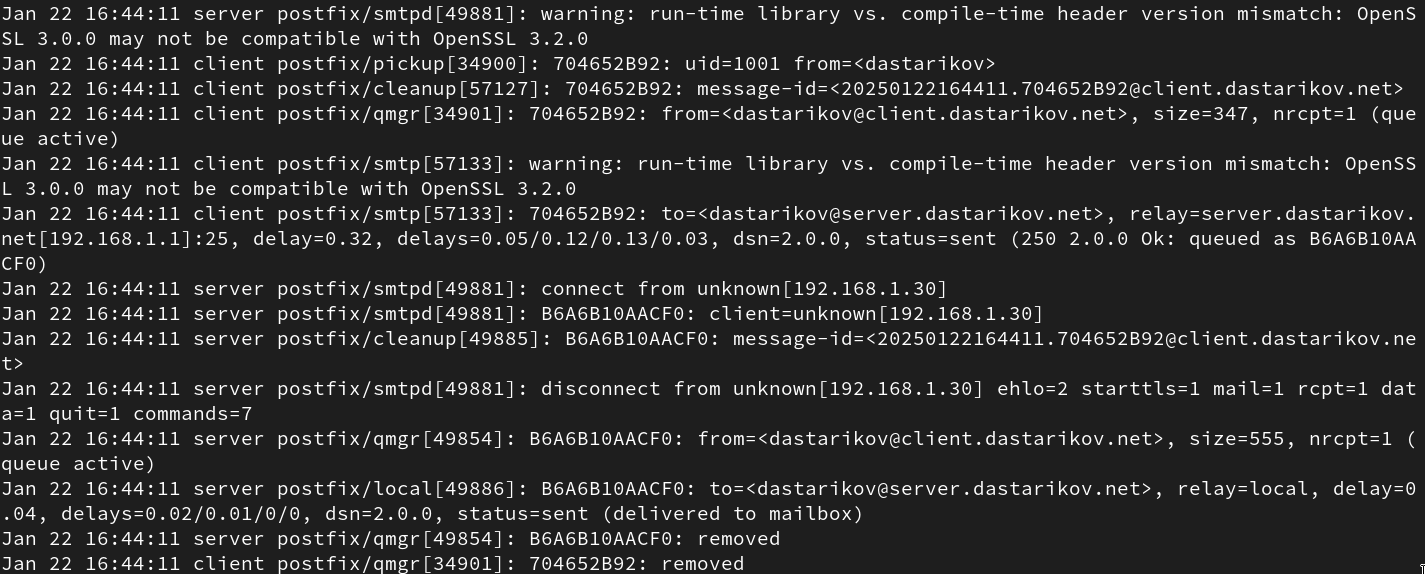
\includegraphics[width=\textwidth]{../images/image19.png}
    \captionof{figure}{Логи при повторной отправке сообщения с клиента.}
\end{frame}
\begin{frame}
\frametitle{Проверка работы Postfix}
    \centering
    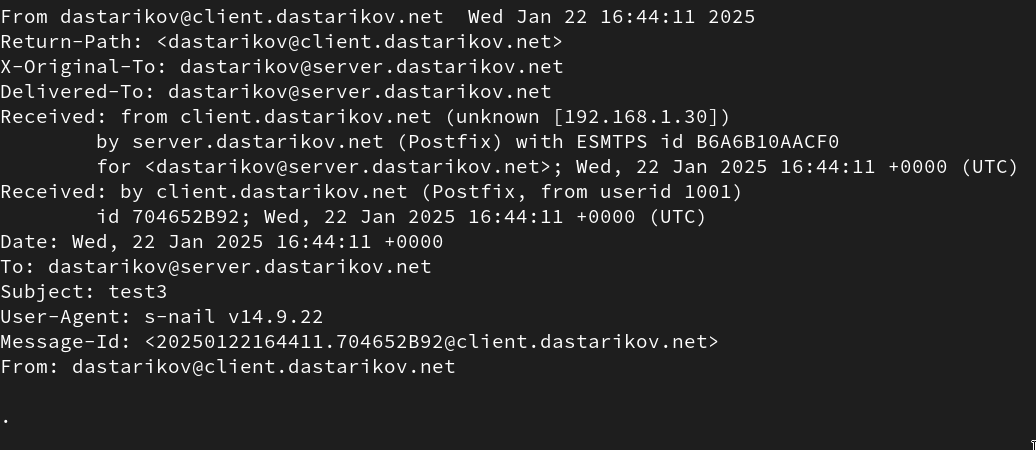
\includegraphics[width=\textwidth]{../images/image20.png}
    \captionof{figure}{Содержимое отправленного  сообщения, хранимое на сервере.}
\end{frame}

\begin{frame}
\frametitle{Конфигурация Postfix для домена}
    \centering
    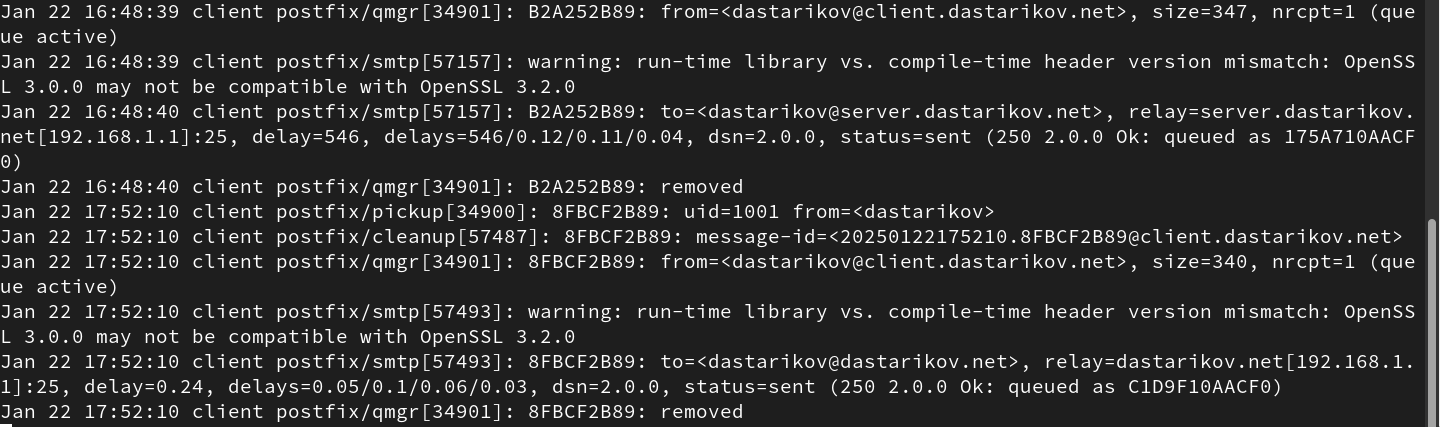
\includegraphics[width=\textwidth]{../images/image21.png}
    \captionof{figure}{Логи при отправке сообщения на доменный адрес.}
\end{frame}
\begin{frame}
\frametitle{Конфигурация Postfix для домена}
    \centering
    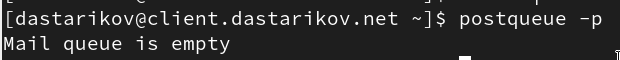
\includegraphics[width=\textwidth]{../images/image22.png}
    \captionof{figure}{Просмотр сообщений в очереди на отправление.}
\end{frame}
\begin{frame}
\frametitle{Конфигурация Postfix для домена}
    \centering
    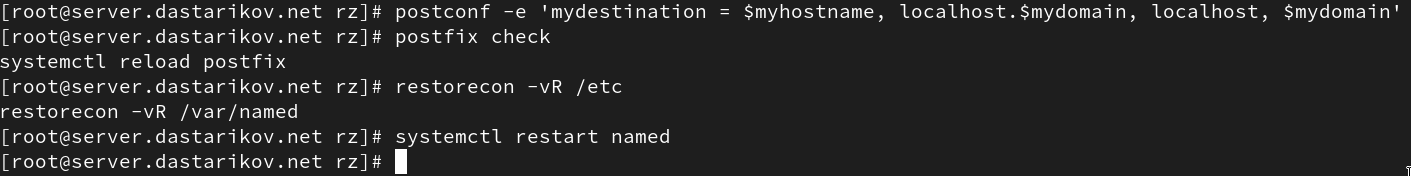
\includegraphics[width=\textwidth]{../images/image25.png}
    \captionof{figure}{Обновление конфигурации Postfix.}
\end{frame}
\begin{frame}
\frametitle{Конфигурация Postfix для домена}
    \centering
    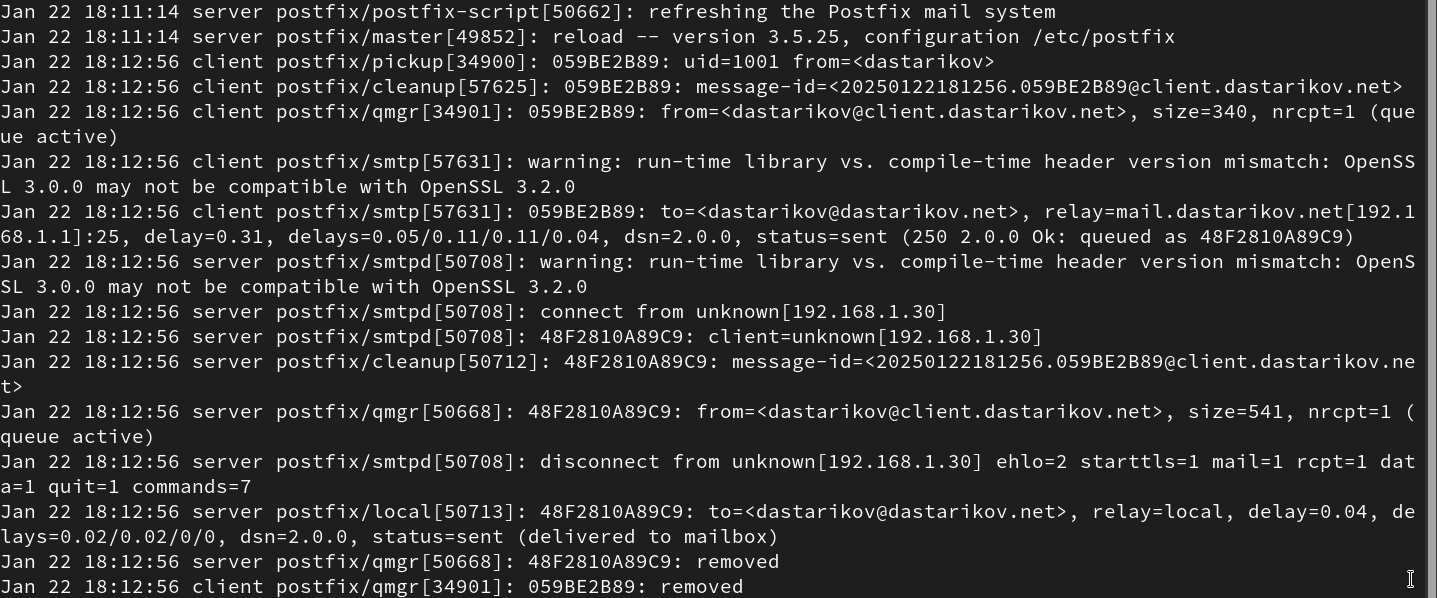
\includegraphics[width=\textwidth]{../images/image26.png}
    \captionof{figure}{Логи при отправке сообщения.}
\end{frame}
\begin{frame}
\frametitle{Конфигурация Postfix для домена}
    \centering
    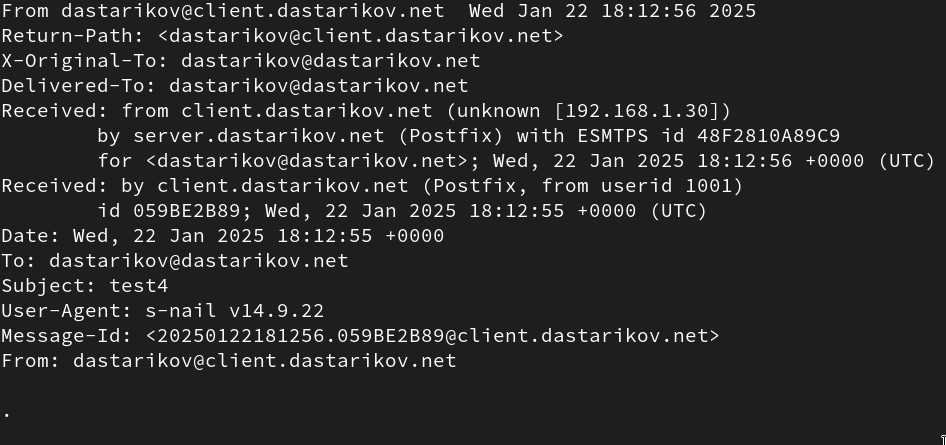
\includegraphics[width=\textwidth]{../images/image27.png}
    \captionof{figure}{Содержание сообщения, хранящееся на сервере.}
\end{frame}
\begin{frame}
\frametitle{Внесение изменений в настройки внутреннего окружения виртуальной машины}
    \centering
    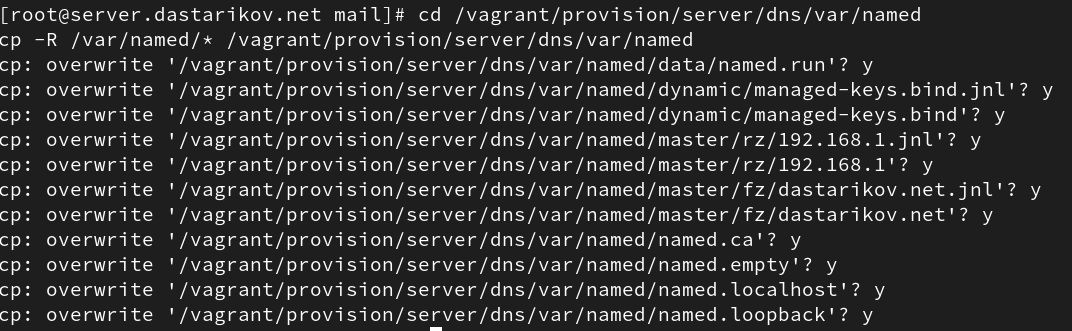
\includegraphics[width=\textwidth]{../images/image28.png}
    \captionof{figure}{Создание каталога для настроек внутреннего окружения.}
\end{frame}
\begin{frame}[containsverbatim]
\frametitle{Внесение изменений в настройки внутреннего окружения виртуальной машины}
\begin{minted}{bash}
  #!/bin/bash
  echo "Provisioning script $0"
  echo "Install needed packages"
  dnf -y install postfix
  dnf -y install s-nail
  echo "Copy configuration files"
  cp -R /vagrant/provision/server/mail/etc/* /etc
  echo "Configure firewall"
  firewall-cmd --add-service=smtp --permanent
  firewall-cmd --reload
  restorecon -vR /etc
  echo "Start postfix service"
  systemctl enable postfix
  systemctl start postfix
\end{minted}
\end{frame}
\begin{frame}[containsverbatim]
\frametitle{Внесение изменений в настройки внутреннего окружения виртуальной машины}
\begin{minted}[breaklines]{bash}
  echo "Configure postfix"
  postconf -e 'mydomain = dastarikov.net'
  postconf -e 'myorigin = $mydomain'
  postconf -e 'inet_protocols = ipv4'
  postconf -e 'inet_interfaces = all'
  postconf -e 'mydestination = $myhostname, localhost.$mydomain, localhost, $mydomain'
  postconf -e 'mynetworks = 127.0.0.0/8, 192.168.0.0/16'
  postfix set-permissions
  restorecon -vR /etc
  systemctl stop postfix
  systemctl start postfix
\end{minted}
\end{frame}
\begin{frame}
\frametitle{Выводы}
\begin{itemize}
    \item В результате выполнения лабораторной работы приобрели практические навыки по установке и конфигурированию SMTP-сервера.
\end{itemize}
\end{frame}
\end{document}
